
%{{第十一回}}{第十一回}}

\chapter{庆寿辰宁府排家宴\hspace{.5em}见熙凤贾瑞起淫心}

{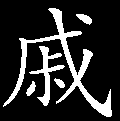
\includegraphics[width=3mm]{../Images/00005}  \kaishu 幻景无端换境生,玉楼春暖述乖情。闹中寻静浑闲事,运得灵机属凤卿。}

话说是日贾敬的寿辰,贾珍先将上等可吃的东西,稀奇些的果品,装了十六大捧盒,着贾蓉带领家下人等与贾敬送去,向贾蓉说道:``你留神看太爷喜欢不喜欢,你就行了礼来。你说:`我父亲遵太爷的话未敢来,在家里率领合家都朝上行了礼了。'''贾蓉听罢,即率领家人去了。

这里渐渐的就有人来了。先是贾琏贾蔷到来,先看了各处的座位,并问:``有什么顽意儿没有?''家人答道:``我们爷原算计请太爷今日来家来,所以未敢预备顽意儿。前日听见太爷又不来了,现叫奴才们找了一班小戏儿并一档子打十番的,都在园子里戏台上预备着呢。''

次后邢夫人、王夫人、凤姐儿、宝玉都来了,贾珍并尤氏接了进去。尤氏的母亲已先在这里呢。大家见过了,彼此让了坐。贾珍尤氏二人亲自递了茶,因说道:``老太太原是老祖宗,我父亲又是侄儿,这样日子,原不敢请他老人家,但是这个时候,天气正凉爽,满园的菊花又盛开,请老祖宗过来散散闷,看着众儿孙热闹热闹,是这个意思。谁知老祖宗又不肯赏脸。''凤姐儿未等王夫人开口,先说道:``老太太昨日还说要来着呢,因为晚上看着宝兄弟他们吃桃儿,老人家又嘴馋,吃了有大半个,五更天的时候就一连起来了两次,{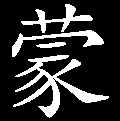
\includegraphics[width=3mm]{../Images/00006}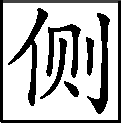
\includegraphics[width=3mm]{../Images/00011}\footnotesize \kaishu 此一问一答,即景生情,请教是真是假?非身经其事者,想不到,写不出。}今日早晨略觉身子倦些。因叫我回大爷,今日断不能来了,说有好吃的要几样,还要很烂的。''{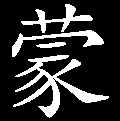
\includegraphics[width=3mm]{../Images/00006}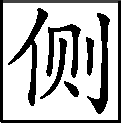
\includegraphics[width=3mm]{../Images/00011}\footnotesize \kaishu 是。}贾珍听了笑道:``我说老祖宗是爱热闹的,今日不来,必定有个原故,若是这么着就是了。''

王夫人道:``前日听见你大妹妹说,蓉哥儿媳妇儿身上有些不大好,到底是怎么样?''尤氏道:``他这个病得的也奇。上月中秋还跟着老太太、太太们顽了半夜,回家来好好的。到了二十后,一日比一日觉懒,也懒待吃东西,这将近有半个多月了。经期又有两个月没来。''邢夫人接着说道:``别是喜罢?''{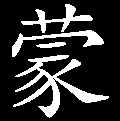
\includegraphics[width=3mm]{../Images/00006}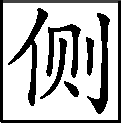
\includegraphics[width=3mm]{../Images/00011}\footnotesize \kaishu 此书总是一幅《云龙图》。}

正说着,外头人回道:``大老爷,二老爷并一家子的爷们都来了,在厅上呢。''贾珍连忙出去了。这里尤氏方说道:``从前大夫也有说是喜的。昨日冯紫英荐了他从学过的一个先生,医道很好,瞧了说不是喜,竟是很大的一个症候。昨日开了方子,吃了一剂药,今日头眩的略好些,别的仍不见怎么样大见效。''凤姐儿道:``我说他不是十分支持不住,今日这样的日子,再也不肯不扎挣着上来。''尤氏道:``你是初三日在这里见他的,他强扎挣了半天,也是因你们娘儿两个好的上头,他才恋恋的舍不得去。''凤姐儿听了,眼圈儿红了半天,半日方说道:``真是`天有不测风云,人有旦夕祸福'。{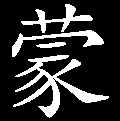
\includegraphics[width=3mm]{../Images/00006}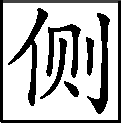
\includegraphics[width=3mm]{../Images/00011}\footnotesize \kaishu 揣摩的极平常言语来写无涯之幻景幻情,反作了悟之意,且又转至别处,真是月下梨花,几不能辨。}这个年纪,倘或就因这个病上怎么样了,人还活着有甚么趣儿!''{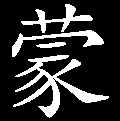
\includegraphics[width=3mm]{../Images/00006}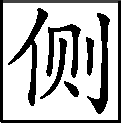
\includegraphics[width=3mm]{../Images/00011}\footnotesize \kaishu 大英雄多在此等处悟得,每能超凡入圣。}正说话间,贾蓉进来,给邢夫人、王夫人、凤姐儿前都请了安,方回尤氏道:``方才我去给太爷送吃食去,并回说我父亲在家中伺候老爷们,款待一家子的爷们,遵太爷的话未敢来。太爷听了甚喜欢,说:`这才是。'叫告诉父亲母亲好生伺候太爷太太们,叫我好生伺候叔叔婶子们并哥哥们。还说那《阴骘文》,叫急急的刻出来,印一万张散人。我将此话都回了我父亲了。我这会子得快出去打发太爷们并合家爷们吃饭。''凤姐儿说:``蓉哥儿,你且站住。你媳妇今日到底是怎么着?''贾蓉皱皱眉说道:``不好么!婶子回来瞧瞧去就知道了。''{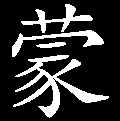
\includegraphics[width=3mm]{../Images/00006}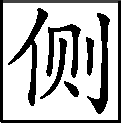
\includegraphics[width=3mm]{../Images/00011}\footnotesize \kaishu 伏线自然。}于是贾蓉出去了。

这里尤氏向邢夫人、王夫人道:``太太们在这里吃饭阿,还是在园子里吃去好?小戏儿现预备在园子里呢。''王夫人向邢夫人道:``我们索性吃了饭再过去罢,也省好些事。''邢夫人道:``很好。''于是尤氏就吩咐媳妇婆子们:``快送饭来。''门外一齐答应了一声,都各人端各人的去了。不多一时,摆上了饭。尤氏让邢夫人、王夫人并他母亲都上了坐,他与凤姐儿、宝玉侧席坐了。邢夫人、王夫人道:``我们来原为给大老爷拜寿,这不竟是我们来过生日来了么?''凤姐儿说道:``大老爷原是好养静的,已经修炼成了,也算得是神仙了。太太们这么一说,这就叫作`心到神知'了。''{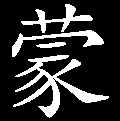
\includegraphics[width=3mm]{../Images/00006}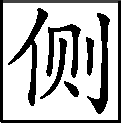
\includegraphics[width=3mm]{../Images/00011}\footnotesize \kaishu 此等趣语,亦不肯无着落。}一句话说的满屋里的人都笑起来了。

于是,尤氏的母亲并邢夫人、王夫人、凤姐儿都吃毕饭,漱了口,净了手,才说要往园子里去,贾蓉进来向尤氏说道:``老爷们并众位叔叔、哥哥、兄弟们也都吃了饭了。大老爷说家里有事,二老爷是不爱听戏又怕人闹的慌,都才去了。别的一家子爷们都被琏二叔并蔷兄弟让过去听戏去了。方才南安郡王、东平郡王、西宁郡王、北静郡王四家王爷,并镇国公牛府等六家,忠靖侯史府等八家,都差人持了名帖送寿礼来,俱回了我父亲,先收在账房里了,礼单都上上档子了。老爷的领谢的名帖都交给各来人了,各来人也都照旧例赏了,众来人都让吃了饭才去了。母亲该请二位太太、老娘、婶子都过园子里坐着去罢。''{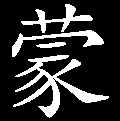
\includegraphics[width=3mm]{../Images/00006}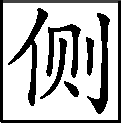
\includegraphics[width=3mm]{../Images/00011}\footnotesize \kaishu 人送寿礼,是为园子;回人去的去了在的在,是为可以过园子里坐;园子里坐,可以转入正文中之幻情;幻情里有乖情,而乖情初写,偏不乖。真是慧心神手!}尤氏道:``也是才吃完了饭,就要过去了。''

凤姐儿说:``我回太太,我先瞧瞧蓉哥儿媳妇,我再过去。''王夫人道:``很是,我们都要去瞧瞧他,倒怕他嫌闹的慌,{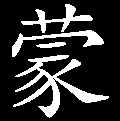
\includegraphics[width=3mm]{../Images/00006}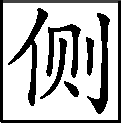
\includegraphics[width=3mm]{../Images/00011}\footnotesize \kaishu 为下文留地步。}说我们问他好罢。''尤氏道:``好妹妹,媳妇听你的话,你去开导开导他,我也放心。你就快些过园子里来。''宝玉也要跟了凤姐儿去瞧秦氏去,王夫人道:``你看看就过去罢,那是侄儿媳妇。''于是尤氏请了邢夫人、王夫人并他母亲都过会芳园去了。

凤姐儿、宝玉方和贾蓉到秦氏这边来。进了房门,悄悄的走到里间房门口,秦氏见了,就要站起来,凤姐儿说:``快别起来,看起猛了头晕。''{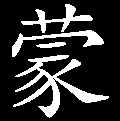
\includegraphics[width=3mm]{../Images/00006}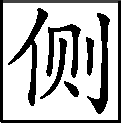
\includegraphics[width=3mm]{../Images/00011}\footnotesize \kaishu 知心每每如此。}于是凤姐儿就紧走了两步,拉住秦氏的手,说道:``我的奶奶!怎么几日不见,就瘦的这么着了!''于是就坐在秦氏坐的褥子上。宝玉也问了好,坐在对面椅子上。贾蓉叫:``快倒茶来,婶子和二叔在上房还未喝茶呢。''

秦氏拉着凤姐儿的手,强笑道:``这都是我没福。这样人家,公公婆婆当自己的女孩儿似的待。{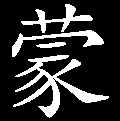
\includegraphics[width=3mm]{../Images/00006}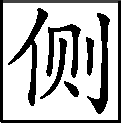
\includegraphics[width=3mm]{../Images/00011}\footnotesize \kaishu 正写幻情,偏作锥心刺骨语。呼渡河者三,是一意。}婶娘的侄儿虽说年轻,却也是他敬我,我敬他,从来没有红过脸儿。就是一家子的长辈同辈之中,除了婶子倒不用说了,别人也从无不疼我的,也无不和我好的。这如今得了这个病,把我那要强的心一分也没了。公婆跟前未得孝顺一天,就是婶娘这样疼我,我就有十分孝顺的心,如今也不能够了。我自想着,未必熬的过年去呢。''

宝玉正眼瞅着那《海棠春睡图》并那秦太虚写的``嫩寒锁梦因春冷,芳气笼人是酒香''的对联,不觉想起在这里睡晌觉梦到``太虚幻境''的事来。正自出神,听得秦氏说了这些话,如万箭攒心,那眼泪不知不觉就流下来了。凤姐儿心中虽十分难过,但恐怕病人见了众人这个样儿反添心酸,倒不是来开导劝解的意思了。见宝玉这个样子,因说道:``宝兄弟,你忒婆婆妈妈的了。他病人不过是这么说,那里就到得这个田地了?况且能多大年纪的人,略病一病儿就这么想那么想的,这不是自己倒给自己添病了么?''贾蓉道:``他这病也不用别的,只是吃得些饮食就不怕了。''{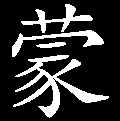
\includegraphics[width=3mm]{../Images/00006}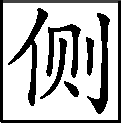
\includegraphics[width=3mm]{../Images/00011}\footnotesize \kaishu 各人是各人伎俩,一丝不乱,一毫不遗。}凤姐儿道:``宝兄弟,太太叫你快过去呢。你别在这里只管这么着,倒招的媳妇也心里不好。太太那里又惦着你。''因向贾蓉说道:``你先同你宝叔叔过去罢,{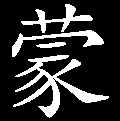
\includegraphics[width=3mm]{../Images/00006}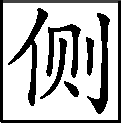
\includegraphics[width=3mm]{../Images/00011}\footnotesize \kaishu 为本。}我还略坐一坐儿。''贾蓉听说,即同宝玉过会芳园来了。

这里凤姐儿又劝解了秦氏一番,又低低的说了许多衷肠话儿,尤氏打发人请了两三遍,凤姐儿才向秦氏说道:``你好生养着罢,我再来看你。合该你这病要好,所以前日就有人荐了这个好大夫来,再也是不怕的了。''秦氏笑道:``任凭神仙也罢,治得病治不得命。婶子,我知道我这病不过是挨日子。''凤姐儿说道:``你只管这么想着,病那里能好呢?总要想开了才是。况且听得大夫说,`若是不治,怕的是春天不好',如今才九月半,还有四五个月的工夫,什么病治不好呢?咱们若是不能吃人参的人家,这也难说了,你公公婆婆听见治得好你,别说一日二钱人参,就是二斤也能够吃的起。好生养着罢,我过园子里去了。''秦氏又道:``婶子,恕我不能跟过去了。闲了时候还求婶子常过来瞧瞧我,咱们娘儿们坐坐,多说几遭话儿。''凤姐儿听了,不觉得又眼圈儿一红,遂说道:``我得了闲儿必常来看你。''于是凤姐儿带领跟来的婆子丫头并宁府的媳妇婆子们,从里头绕进园子的便门来。{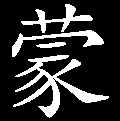
\includegraphics[width=3mm]{../Images/00006}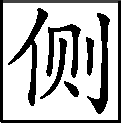
\includegraphics[width=3mm]{../Images/00011}\footnotesize \kaishu 偏不独行,用此等反克文字。}但只见:

黄花满地,白柳横坡。小桥通若耶之溪,曲径接天台之路。{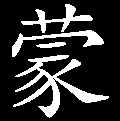
\includegraphics[width=3mm]{../Images/00006}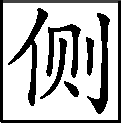
\includegraphics[width=3mm]{../Images/00011}\footnotesize \kaishu 点明题目。}石中清流激湍,篱落飘香;树头红叶翩翻,疏林如画。西风乍紧,初罢莺啼;暖日当暄,又添蛩语。遥望东南,建几处依山之榭;纵观西北,结三间临水之轩。笙簧盈耳,别有幽情;罗绮穿林,倍添韵致。

凤姐儿正自看园中景致,一步步行来赞赏。猛然从假山石后走过一个人来,向前对凤姐儿说道:``请嫂子安。''凤姐儿猛然见了,将身子望后一退,说道:``这是瑞大爷不是?''贾瑞说道:``嫂子连我也不认得了?不是我是谁!''凤姐儿道:``不是不认得,猛然一见,不想到是大爷到这里来。''{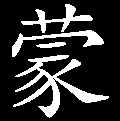
\includegraphics[width=3mm]{../Images/00006}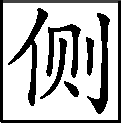
\includegraphics[width=3mm]{../Images/00011}\footnotesize \kaishu 作者何等心思,能在此等事想到如此出言。渐入之妙,无过于此。}贾瑞道:``也是合该我与嫂子有缘。我方才偷出了席,在这个清净地方略散一散,不想就遇见嫂子也从这里来。这不是有缘么?''{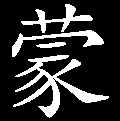
\includegraphics[width=3mm]{../Images/00006}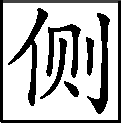
\includegraphics[width=3mm]{../Images/00011}\footnotesize \kaishu 重点``有缘''二字,方是笔力。}一面说着,一面拿眼睛不住的觑着凤姐儿。

凤姐儿是个聪明人,见他这个光景,如何不猜透八九分呢,因向贾瑞假意含笑道:``怨不得你哥哥时常提你,说你很好。今日见了,听你说这几句话儿,就知道你是个聪明和气的人了。这会子我要到太太们那里去,不得和你说话儿,等闲了咱们再说话儿罢。''贾瑞道:``我要到嫂子家里去请安,又恐怕嫂子年轻,不肯轻易见人。''凤姐儿假意笑道:``一家子骨肉,说什么年轻不年轻的话。''贾瑞听了这话,再不想到今日得这个奇遇,那神情光景亦发不堪难看了。凤姐儿说道:``你快入席去罢,仔细他们拿住罚你酒。''贾瑞听了,身上已木了半边,慢慢的一面走着,一面回过头来看。凤姐儿故意的把脚步放迟了些儿,见他去远了,心里暗忖道:``这才是知人知面不知心呢,那里有这样禽兽的人呢!{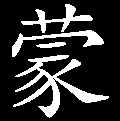
\includegraphics[width=3mm]{../Images/00006}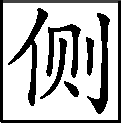
\includegraphics[width=3mm]{../Images/00011}\footnotesize \kaishu 大英雄气概。作者以此命凤,其有为耶?}他如果如此,几时叫他死在我的手里,他才知道我的手段!''

于是凤姐儿方移步前来。将转过了一重山坡,见两三个婆子慌慌张张的走来,见了凤姐儿,笑说道:``我们奶奶见二奶奶只是不来,急的了不得,叫奴才们又来请奶奶来了。''{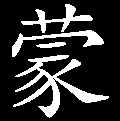
\includegraphics[width=3mm]{../Images/00006}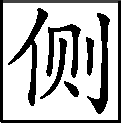
\includegraphics[width=3mm]{../Images/00011}\footnotesize \kaishu 别者必将遇贾瑞的事声张一番,以表清节。此文偏若无事,一则可以见熙凤非凡,一则可以见熙凤包含广大。}凤姐儿说道:``你们奶奶就是这么急脚鬼似的。''凤姐儿慢慢的走着,问:``戏唱了几出了?''那婆子回道:``有八九出了。''说话之间,已来到了天香楼的后门,见宝玉和一群丫头们在那里玩呢。凤姐儿说道:``宝兄弟,别忒淘气了。''{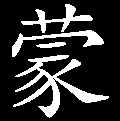
\includegraphics[width=3mm]{../Images/00006}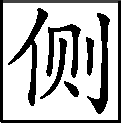
\includegraphics[width=3mm]{../Images/00011}\footnotesize \kaishu 照应前文。}有一个丫头说道:``太太们都在楼上坐着呢,请奶奶就从这边上去罢。''

凤姐儿听了,款步提衣上了楼,见尤氏已在楼梯口等着呢。尤氏笑说道:``你们娘儿两个忒好了,见了面总舍不得来了。你明日搬来和他住着罢。你坐下,我先敬你一钟。''于是凤姐儿在邢、王二夫人前告了坐,又在尤氏的母亲前周旋了一遍,仍同尤氏坐在一桌上吃酒听戏。尤氏叫拿戏单来,让凤姐儿点戏,凤姐儿说道:``亲家太太和太太们在这里,我如何敢点。''邢夫人、王夫人说道:``我们和亲家太太都点了好几出了,你点两出好的我们听。''凤姐儿立起身来答应了一声,方接过戏单,从头一看,点了一出《还魂》,一出《弹词》,递过戏单去说:``现在唱的这《双官诰》,{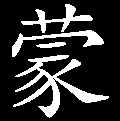
\includegraphics[width=3mm]{../Images/00006}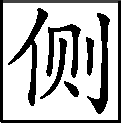
\includegraphics[width=3mm]{../Images/00011}\footnotesize \kaishu 点下文。}唱完了,再唱这两出,也就是时候了。''王夫人道:``可不是呢,也该趁早叫你哥哥嫂子歇歇,他们又心里不静。''尤氏说道:``太太们又不常过来,娘儿们多坐一会子去,才有趣儿,天还早呢。''凤姐儿立起身来望楼下一看,说:``爷们都往那里去了?''旁边一个婆子道:``爷们才到凝曦轩,带了打十番的那里吃酒去了。''凤姐儿说道:``在这里不便宜,背地里又不知干什么去了!''{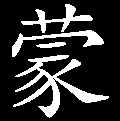
\includegraphics[width=3mm]{../Images/00006}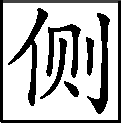
\includegraphics[width=3mm]{../Images/00011}\footnotesize \kaishu 偏是爱吃酸醋。}尤氏笑道:``那里都像你这么正经人呢。''

于是说说笑笑,点的戏都唱完了,方才撤下酒席,摆上饭来。吃毕,大家才出园子来,到上房坐下,吃了茶,方才叫预备车,向尤氏的母亲告了辞。尤氏率同众姬妾并家下婆子媳妇们方送出来,贾珍率领众子侄都在车旁侍立,等候着呢,见了邢夫人、王夫人道:``二位婶子明日还过来逛逛。''王夫人道:``罢了,我们今日整坐了一日,也乏了,明日歇歇罢。''于是都上车去了。贾瑞犹不时拿眼睛觑着凤姐儿。{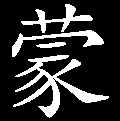
\includegraphics[width=3mm]{../Images/00006}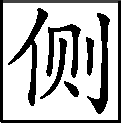
\includegraphics[width=3mm]{../Images/00011}\footnotesize \kaishu 无有不足不尽处。}贾珍等进去后,李贵才拉过马来,宝玉骑上,随了王夫人去了。这里贾珍同一家子的弟兄子侄吃过了晚饭,方大家散了。

次日,仍是众族人等闹了一日,不必细说。此后,凤姐儿不时亲自来看秦氏。秦氏也有几日好些,也有几日仍是那样。贾珍、尤氏、贾蓉好不焦心。{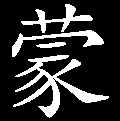
\includegraphics[width=3mm]{../Images/00006}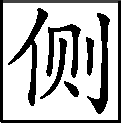
\includegraphics[width=3mm]{../Images/00011}\footnotesize \kaishu 陪衬补足。}

且说贾瑞到荣府来了几次,偏都遇见凤姐儿往宁府那边去了。这年正是十一月三十日冬至。到交节的那几日,贾母、王夫人、凤姐儿日日差人去看秦氏,回来的人都说:``这几日也没见添病,也不见甚好。''王夫人向贾母说:``这个症候,遇着这样大节不添病,就有好大的指望了。''贾母说:``可是呢,好个孩子,要是有些原故,可不叫人疼死。''说着,一阵心酸,叫凤姐儿说道:``你们娘儿两个也好了一场,明日大初一,过了明日,你后日再去看一看他去。你细细的瞧瞧他那光景,倘或好些儿,你回来告诉我,我也喜欢喜欢。那孩子素日爱吃的,你也常叫人做些给他送过去。''凤姐儿一一的答应了。

到了初二日,吃了早饭,来到宁府,看见秦氏的光景,虽未甚添病,但是那脸上身上的肉全瘦干了。于是和秦氏坐了半日,说了些闲话儿,又将这病无妨的话开导了一遍。秦氏说道:``好不好,春天就知道了。如今现过了冬至,又没怎么样,或者好的了也未可知。婶子回老太太、太太放心罢。{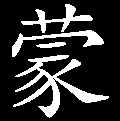
\includegraphics[width=3mm]{../Images/00006}\includegraphics[width=3mm]{../Images/00011}\footnotesize \kaishu 文字一变。人于将死时也应有一变。}昨日老太太赏的那枣泥馅的山药糕,我倒吃了两块,倒像克化的动似的。''凤姐儿说道:``明日再给你送来。我到你婆婆那里瞧瞧,就要赶着回去回老太太的话去。''秦氏道:``婶子替我请老太太、太太安罢。''

凤姐儿答应着就出来了,到了尤氏上房坐下。尤氏道:``你冷眼瞧媳妇是怎么样?''凤姐儿低了半日头,说道:``这实在没法儿了。你也该将一应的后事用的东西给他料理料理,冲一冲也好。''{\includegraphics[width=3mm]{../Images/00006}\includegraphics[width=3mm]{../Images/00011}\footnotesize \kaishu 伏下文代办理丧事。}尤氏道:``我也叫人暗暗的预备了。就是那件东西不得好木头,暂且慢慢的办罢。''于是凤姐儿吃了茶,说了一会子话儿,说道:``我要快回去回老太太的话去呢。''尤氏道:``你可缓缓的说,别吓着老太太。''凤姐儿道:``我知道。''于是凤姐儿就回来了。到了家中,见了贾母,说:``蓉哥儿媳妇请老太太安,给老太太磕头,说他好些了,求老祖宗放心罢。他再略好些,还要给老祖宗磕头请安来呢。''贾母道:``你看他是怎么样?''凤姐儿说:``暂且无妨,精神还好呢。''{\includegraphics[width=3mm]{../Images/00006}\includegraphics[width=3mm]{../Images/00011}\footnotesize \kaishu ``精神还好呢''五字,写得出神入化。}贾母听了,沉吟了半日,因向凤姐儿说:``你换换衣服歇歇去罢。''

凤姐儿答应着出来,见过了王夫人,到了家中,平儿将烘的家常的衣服给凤姐儿换了。凤姐儿方坐下,问道:``家里没有什么事么?''平儿方端了茶来,递了过去,说道:``没有什么事。就是那三百银子的利银,旺儿媳妇送进来,我收了。{\includegraphics[width=3mm]{../Images/00006}\includegraphics[width=3mm]{../Images/00011}\footnotesize \kaishu 陪。}再有瑞大爷使人来打听{\includegraphics[width=3mm]{../Images/00006}\includegraphics[width=3mm]{../Images/00011}\footnotesize \kaishu 正。}奶奶在家没有,他要来请安说话。''凤姐儿听了,``哼''了一声,说道:``这畜生合该作死,看他来了怎么样!''平儿因问道:``这瑞大爷是因什么只管来?''凤姐儿遂将九月里宁府园子里遇见他的光景,他说的话,都告诉了平儿。平儿说道:``癞蛤蟆想天鹅肉吃,没人伦的混帐东西,起这个念头,叫他不得好死!''凤姐儿道:``等他来了,我自有道理。''不知贾瑞来时作何光景,且听下回分解。

{\includegraphics[width=3mm]{../Images/00005}  \kaishu  总评:将可卿之病将死,作幻情一劫;又将贾瑞之遇唐突,作幻情一变。下回同归幻境,真风马牛不相及之谈。同范并趋,毫无滞碍,灵活之至,飘飘欲仙。默思作者其人之心,其人之形,其人之神,其人之文,必宋玉、子建一般心性,一流人物。}

